\documentclass[tikz,border=5mm]{standalone}

\usepackage[T1]{fontenc}
\usepackage[sfdefault,sb]{plex-sans}
\usepackage{xcolor}
\usepackage{tikz}

\usetikzlibrary{calc,positioning}

\pgfdeclarelayer{bg}
\pgfsetlayers{bg,main}

\renewcommand*\familydefault{\sfdefault}
\hyphenpenalty=10000
\exhyphenpenalty=10000

\definecolor{foundationfill}{HTML}{2E64FE}
\definecolor{foundationstroke}{HTML}{153E7E}
\definecolor{corefill}{HTML}{0033CC}
\definecolor{corestroke}{HTML}{001F7A}
\definecolor{advancedfill}{HTML}{000066}
\definecolor{advancedstroke}{HTML}{000033}
\definecolor{edgegray}{HTML}{475569}
\definecolor{optionalfill}{HTML}{EAF0FF}
\definecolor{optionalstroke}{HTML}{153E7E}

\begin{document}
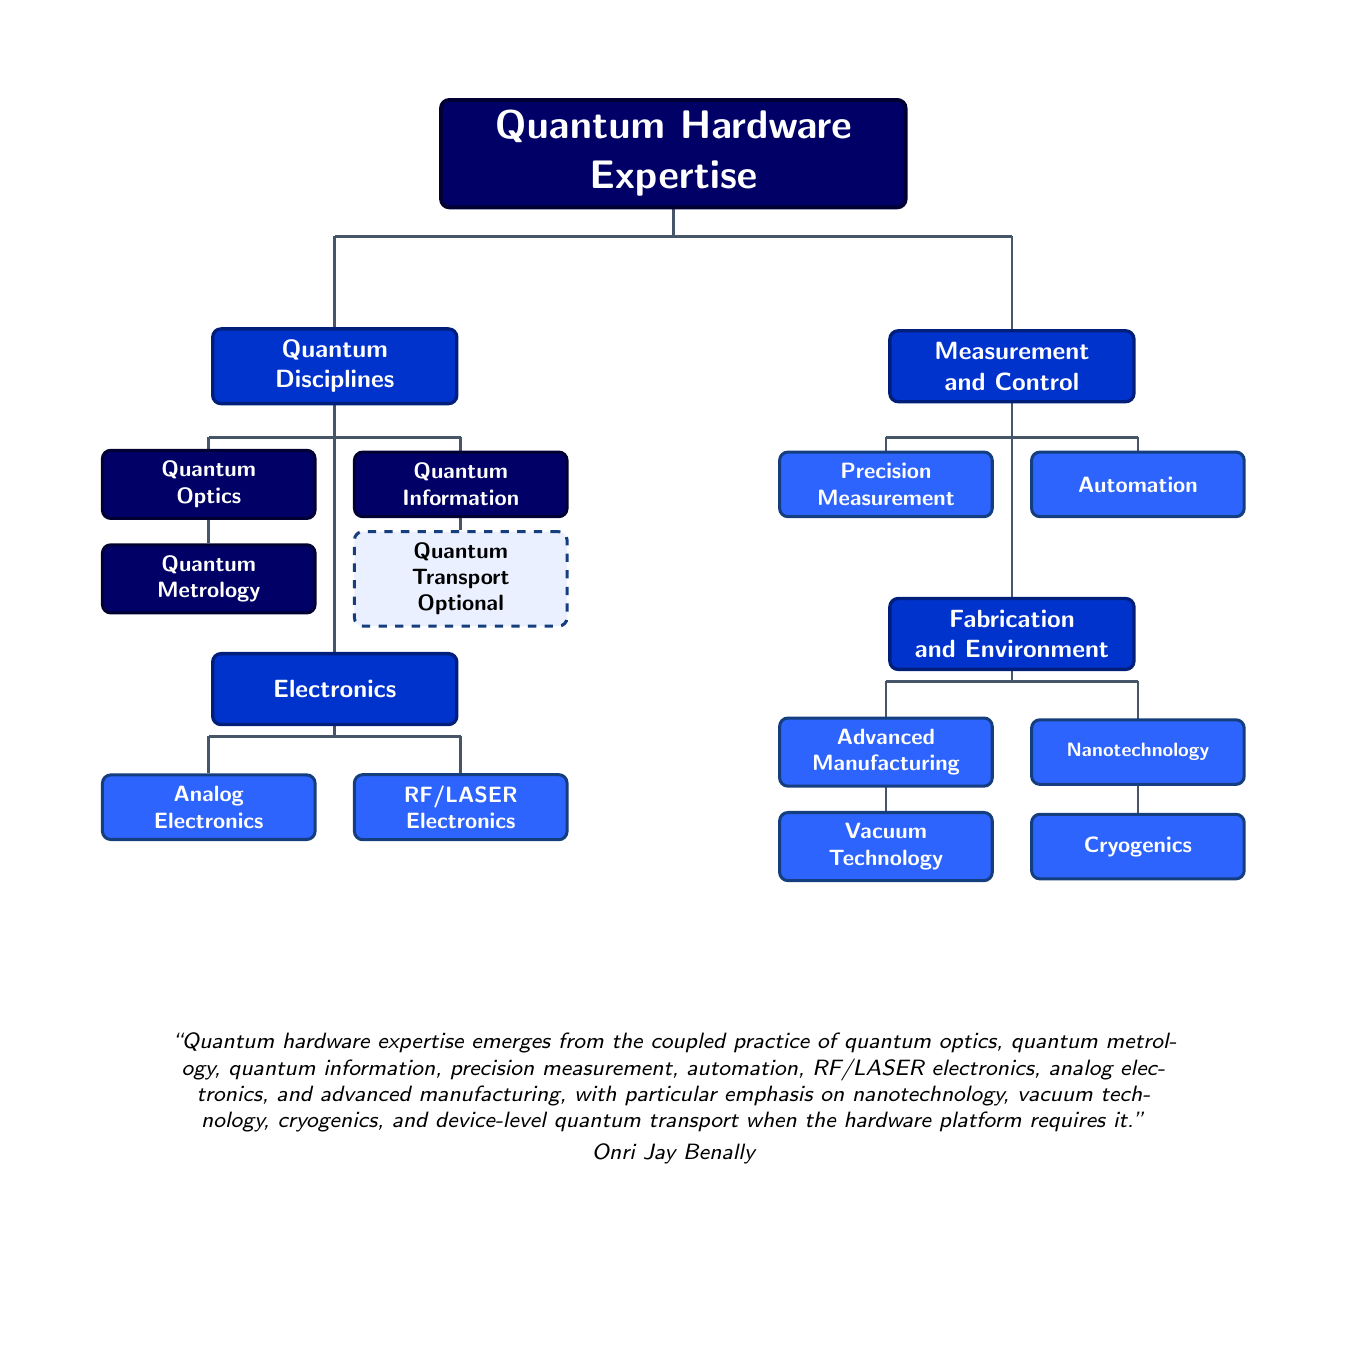
\begin{tikzpicture}[
  x=1cm,
  y=1cm,
  branch/.style={
    draw=edgegray,
    line width=1.0pt
  },
  every node/.style={
    rectangle,
    rounded corners=3pt,
    align=center,
    inner sep=4pt,
    font=\small
  },
  root/.style={
    draw=advancedstroke,
    fill=advancedfill,
    text=white,
    line width=1.4pt,
    font=\bfseries\Large,
    minimum width=5.9cm,
    minimum height=1.05cm,
    text width=5.4cm
  },
  category/.style={
    draw=corestroke,
    fill=corefill,
    text=white,
    line width=1.2pt,
    font=\bfseries\small,
    minimum width=3.1cm,
    minimum height=0.90cm,
    text width=2.8cm
  },
  leaf/.style={
    draw=foundationstroke,
    fill=foundationfill,
    text=white,
    line width=1.1pt,
    font=\bfseries\footnotesize,
    minimum width=2.7cm,
    minimum height=0.82cm,
    text width=2.35cm
  },
  leafsmall/.style={
    draw=foundationstroke,
    fill=foundationfill,
    text=white,
    line width=1.1pt,
    font=\bfseries\scriptsize,
    minimum width=2.7cm,
    minimum height=0.82cm,
    text width=2.35cm
  },
  quantumleaf/.style={
    draw=advancedstroke,
    fill=advancedfill,
    text=white,
    line width=1.1pt,
    font=\bfseries\footnotesize,
    minimum width=2.7cm,
    minimum height=0.82cm,
    text width=2.35cm
  },
  optional/.style={
    draw=optionalstroke,
    fill=optionalfill,
    text=black,
    dashed,
    line width=1.1pt,
    font=\bfseries\footnotesize,
    minimum width=2.7cm,
    minimum height=0.82cm,
    text width=2.35cm
  },
  quote/.style={
    draw=none,
    align=center,
    font=\footnotesize\itshape,
    text width=13.5cm
  }
]

\path[use as bounding box] (-8.2,-8.2) rectangle (8.2,8.2);

% Root
\node[root] (qhw) at (0,6.6) {Quantum Hardware\\Expertise};

% Category nodes
\node[category] (qdisc) at (-4.3,3.9) {Quantum\\Disciplines};
\node[category] (meas)  at (4.3,3.9)  {Measurement\\and Control};
\node[category] (elec)  at (-4.3,-0.20) {Electronics};
\node[category] (fab)   at (4.3,0.5)  {Fabrication\\and Environment};

% Leaves for Quantum Disciplines
\node[quantumleaf] (qo) at (-5.9,2.4) {Quantum\\Optics};
\node[quantumleaf] (qi) at (-2.7,2.4) {Quantum\\Information};
\node[quantumleaf] (qm) at (-5.9,1.2) {Quantum\\Metrology};
\node[optional]    (qt) at (-2.7,1.2) {Quantum\\Transport\\Optional};

% Leaves for Measurement and Control
\node[leaf] (pm)   at (2.7,2.4) {Precision\\Measurement};
\node[leaf] (auto) at (5.9,2.4) {Automation};

% Leaves for Electronics
\node[leaf] (analog) at (-5.9,-1.70) {Analog\\Electronics};
\node[leaf] (rf)     at (-2.7,-1.70) {RF/LASER\\Electronics};

% Leaves for Fabrication and Environment
\node[leaf]      (mfg)  at (2.7,-1.0) {Advanced\\Manufacturing};
\node[leafsmall] (nano) at (5.9,-1.0) {Nanotechnology};
\node[leaf]      (vac)  at (2.7,-2.2) {Vacuum\\Technology};
\node[leaf]      (cryo) at (5.9,-2.2) {Cryogenics};

\begin{pgfonlayer}{bg}

% Root branch bus
\coordinate (rootbus) at (0,5.55);
\draw[branch] (qhw.south) -- (rootbus);
\draw[branch] (-4.3,5.55) -- (4.3,5.55);
\draw[branch] (qdisc.north) -- (-4.3,5.55);
\draw[branch] (meas.north)  -- (4.3,5.55);
\draw[branch] (elec.north)  -- (-4.3,5.55);
\draw[branch] (fab.north)   -- (4.3,5.55);

% Quantum Disciplines
\coordinate (qdbus) at (-4.3,3.0);
\draw[branch] (qdisc.south) -- (qdbus);
\draw[branch] (-5.9,3.0) -- (-2.7,3.0);
\draw[branch] (qo.north) -- (-5.9,3.0);
\draw[branch] (qi.north) -- (-2.7,3.0);
\draw[branch] (qm.north) |- (-5.9,3.0);
\draw[branch] (qt.north) |- (-2.7,3.0);

% Measurement and Control
\coordinate (measbus) at (4.3,3.0);
\draw[branch] (meas.south) -- (measbus);
\draw[branch] (2.7,3.0) -- (5.9,3.0);
\draw[branch] (pm.north) -- (2.7,3.0);
\draw[branch] (auto.north) -- (5.9,3.0);

% Electronics
\coordinate (elecbus) at (-4.3,-0.80);
\draw[branch] (elec.south) -- (elecbus);
\draw[branch] (-5.9,-0.80) -- (-2.7,-0.80);
\draw[branch] (analog.north) -- (-5.9,-0.80);
\draw[branch] (rf.north) -- (-2.7,-0.80);

% Fabrication and Environment
\coordinate (fabbus) at (4.3,-0.1);
\draw[branch] (fab.south) -- (fabbus);
\draw[branch] (2.7,-0.1) -- (5.9,-0.1);
\draw[branch] (mfg.north) -- (2.7,-0.1);
\draw[branch] (nano.north) -- (5.9,-0.1);
\draw[branch] (vac.north) |- (2.7,-0.1);
\draw[branch] (cryo.north) |- (5.9,-0.1);

\end{pgfonlayer}

% Quote attribution
\node[quote] at (0,-5.4)
{``Quantum hardware expertise emerges from the coupled practice of quantum optics, quantum metrology, quantum information, precision measurement, automation, RF/LASER electronics, analog electronics, and advanced manufacturing, with particular emphasis on nanotechnology, vacuum technology, cryogenics, and device-level quantum transport when the hardware platform requires it.''\\[2pt]
Onri Jay Benally};

\end{tikzpicture}
\end{document}
